\documentclass[a4paper,11pt]{article}
\usepackage{xcolor}
\usepackage{tikz}
\usetikzlibrary{shapes.arrows,arrows.meta}
\begin{document}
\begin{figure}[h!]
    \centering
    \scalebox{0.1}{
    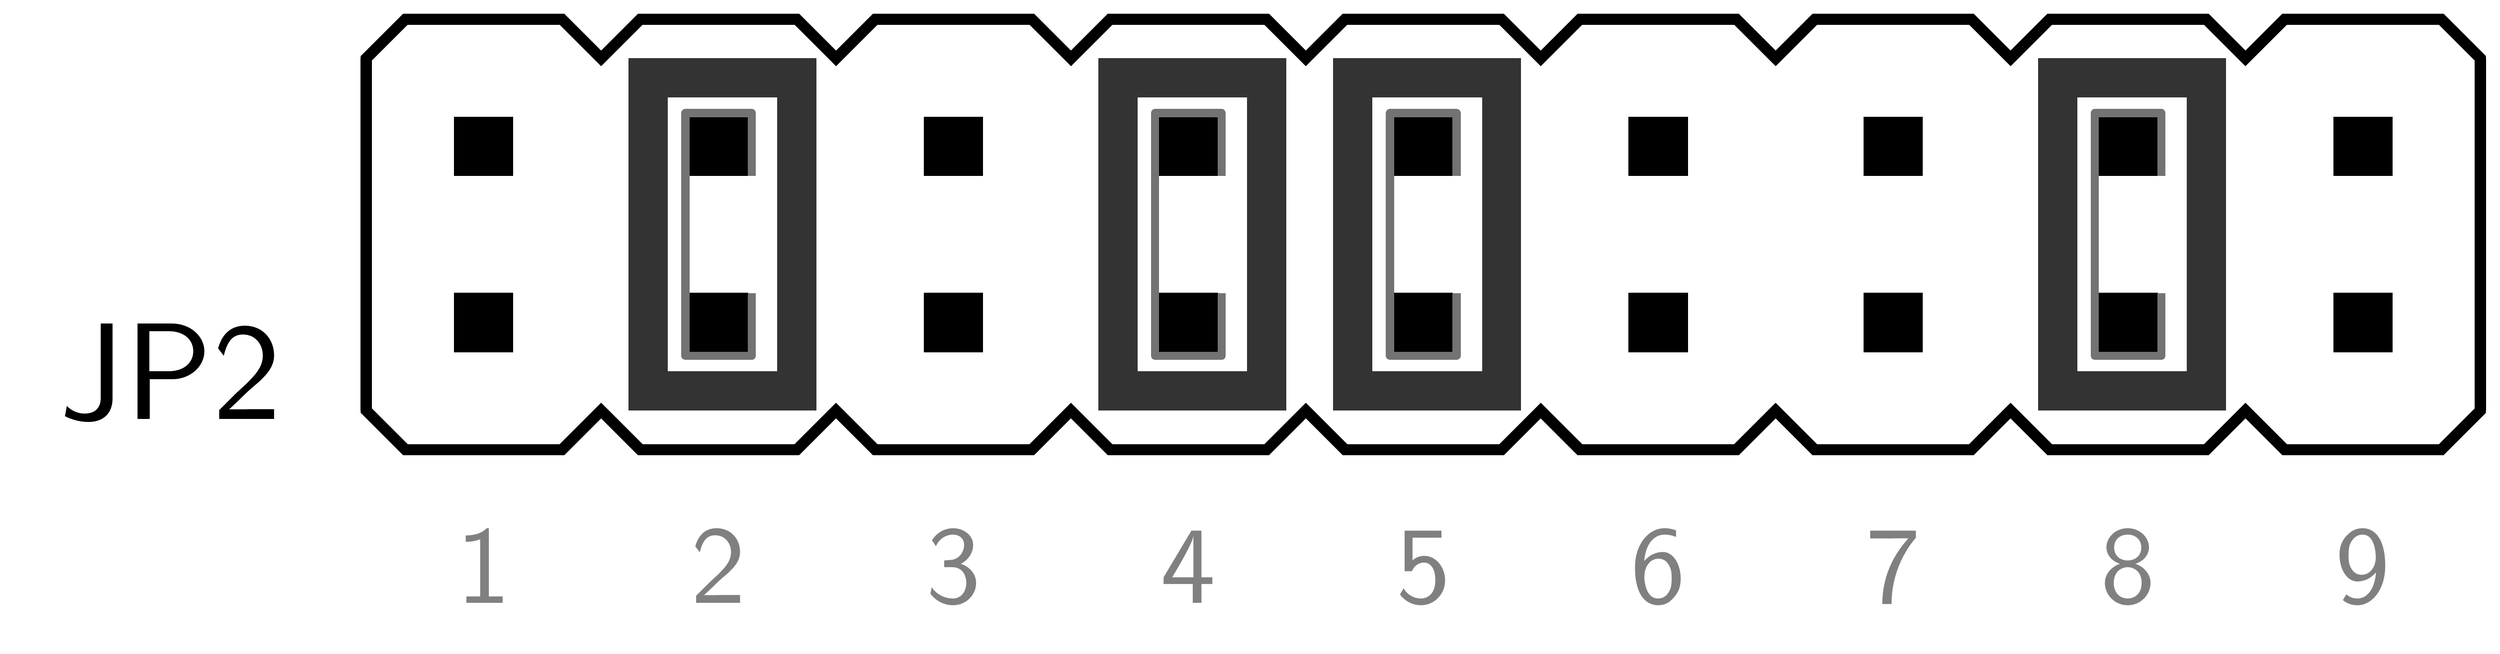
\begin{tikzpicture}[font=\sffamily]
    	\draw [line width=8] (6,4) -- ++(0,9);
    	\draw [line width=8] (60,4) -- ++(0,9);
    	\draw [line width=8] (6,13)
 	\foreach \q in {1, ..., 9} { -- ++(1,1) -- ++(4,0) -- ++(1,-1) } -- ++(0,-9)
	\foreach \q in {9, ..., 1} {	-- ++(-1,-1) -- ++(-4,0) -- ++(-1,1) } -- cycle;
	\foreach \q in {9, ..., 1} {
		\draw [fill=black] (\q*6+2.25,5.5) rectangle ++(1.5,1.5);
 		\draw [fill=black] (\q*6+2.25,10) rectangle ++(1.5,1.5);
		\draw (3+\q*6, 0) node[scale=8,color=gray]{\q};   		
  	}   	
  	\foreach \q in {2,4,5,8} {
  		\draw [line width=6,color=black!55,line join=round] (\q*6+3.85,10) -- ++(0,1.6) -- ++(-1.7,0) -- ++(0,-6.2) -- ++(1.7,0) -- ++(0,1.6);  
  		\draw [line width=1cm, color=black!80] (\q*6+1.2,4.5) rectangle ++(3.8,8);
  	}
	\draw (1,5) node[scale=10]{JP2};   		 	
    \end{tikzpicture}
    }
    \caption{Clock configuration example}
    \label{fig:clkconfig}
\end{figure}
\end{document} 



